\chapter{Experimental Setup}
\label{chp:experimental_setup}
In this chapter we will look at the equipment we use in our recordings.
Further we will go into detail about the limitations and possibilities introduced by this setup, and discuss alternative approaches.


\section{Recording and Sampling}\label{chp3:sec:microphone_selection}

\subsection{Sampling and Encoding}
We want to analyze the acoustic emanations from a \gls{CPU} in the frequency domain, and look at power spectra representing a period of time.
The sampling frequency has a big impact on the range of frequencies that can be analyzed, as it is limited by the Nyquist frequency given in~\autoref{eq:nyquist_frequency}.
Genkin et al. presented results that suggest that one should be able to observe phenomenons related to acoustic emanations from computer systems for frequencies below \(100\)kHz; our setup relies on \gls{NI} myDAQ that is capable of sampling at a rate \({F_{s}}\) of \(200\)kHz~\footnotemark.
Thus by only looking at~\autoref{eq:nyquist_frequency}, we are able to analyze frequencies up to \(100\)kHz.

\footnotetext{Our initial experiments were conducted using a Zoom H4n recorder, with a 96kHz sampling rate. 
However, we did not possess a remote control for the recorder, hence we had to physically press buttons on the recorder to start and stop recordings. 
This introduced a lot of noise in the recordings, and made our results inconclusive.}


\begin{equation}\label{eq:nyquist_frequency}
F_{nc} = \frac{F_{s}}{2}
\end{equation}

The captured signals are stored in WAV files where the audio is encoded as \gls{PCM}.
Hence we do not perform real-time analysis, as we work on stored recordings during our analysis.
Implications are discussed in detail in~\autoref{chp4:predictable_execution}.


\subsection{Portable Recording Setup}\label{chp3:sec:knowles_configuration}
For our first round of experiments we use the Knowles Ultrasonic SPU0410LR5H microphone.
The microphone has a flat frequency response up to 80kHz, with a -4dB sensitivity~\cite{url:knowles_spec}.
To power the microphone we use a 4.5V battery.
\gls{NI} myDAQ is used for sampling, connecting the microphone directly into the Analog Input 0 on the myDAQ device.

The fact that the sampled signal is not bandlimited, i.e there are no low-pass filter in this setup, the sampling theorem suggest that we should observe distortion due to aliasing~\cite[pp. 384-394]{proakis2007digital}.

There are interesting implications of this setup; the microphone itself is very small as well as being very cheap, costing only a few dollars. 
Hence, this is a very portable setup, that can be hidden and used in covert operations against unsuspecting targets, for instance in a side-channel attack against a vulnerable RSA implementation, as suggested in~\cite{DBLP:conf/crypto/GenkinST14}.
The low cost of the parts used, less the myDAQ, also makes it disposable.
A small microphone also enables the possibility to hide the whole setup inside the casing of a desktop computer or a server, thus possibly making side channel attacks easier because of a better signal-to-noise ratio due to reducing the distance between the source and the microphone.


\subsection{Lab Grade Recording Setup}\label{chp3:sec:bruel_kjaer_configuration}
With our second setup we are aiming to come close to what Genkin et al. used for their lab-grade setup.
We use a Brüel\&Kjær 4939 microphone that is able to do precise measurements up to frequencies around 100kHz~\cite{url:bk4939_spec}.
The microphone is then connected to a Norsonic 1201 preamplifier~\cite{url:norsonic1201_spec} which again is connected to a Norsonic type 336 microphone amplifier and power supply.
The Norsonic 336 provides several options regarding the gain~\cite{url:nor336_spec}. 
We use 40 dB gain in all of our recordings.
The output signal from the Norsonic is led into a Krohn-Hite Corporation 3945 filter~\cite{url:krohn-hite3945_spec} which provides a 1kHz high-pass filter as well as a 80kHz low-pass filter.
The filtered signal is sent to the \gls{NI} myDAQ, and lastly encoded in a WAV file using a laptop computer. 

\begin{equation}\label{eq:sampling_theorem}
B \leq \frac{F_{s}}{2}
\end{equation}

The sampling theorem, given in~\autoref{eq:sampling_theorem}, gives that the ability to uniquely recover frequencies $B$ from a sampled signal is bound by the sampling frequency, given a bandlimited continuous-time signal~\cite[pp. 384-394]{proakis2007digital}.
Since the inclusion of a band-pass filter gives such a signal for this setup, and we have $B = 80kHz$ and $F_s = 200kHz$, the condition of the sampling theorem holds.
Thus, we should experience far less distortion resulting from aliasing using this setup.


\section{Processing and Signal Extraction}\label{chp3:sec:processing_signal_extraction}
The captured sound is stored in a WAV file.
This file is processed in using a piece of self written software, which utilizes libraries such as \texttt{FFTW}\footnote{\texttt{FFTW} is a library for computing the Fast Fourier Transform, available at \url{http://www.fftw.org/}} and \texttt{libsndfile}\footnotemark{} to ensure correct processing of the sound files.
%The samples are divided into windows \( W \), where \( \lvert W \rvert = 2^{n} \) where \( n \) is a non-zero positive integer.

\footnotetext{\texttt{libsndfile} is a library for working with different sound file formats, available at \url{http://www.mega-nerd.com/libsndfile/}}

The WAV files produced by the setups explained in this chapter contain a mono signal. 
In the WAV format, frames representing each sample is stored subsequently, such that the sample \( s_{f,c} \) represents the \gls{PCM} response for frame \( f \) channel \( c \).
For a stereo signal this means that \( f \in \left [ 1, 2 \right ] \), thus the samples are ordered  \( s_{0,0}, s_{0,1}, s_{1,0}, s_{1,1}, ... , s_{n,0}, s_{n,1} \).
Since we want to work on a mono signal, we simply ignore all frames where \( f \neq 0 \), which with our setup means that we use all frames in the stored file.

The captured signal is Fourier-transformed using a window size of 4096 frames, and the hamming window function. The power spectra results are studied, with emphasis on how they are evolving in the time domain, and how they correlate to the expected effects of the software described in \autoref{chp4:predictable_execution}.
Source code for these steps are included in~\autoref{apx:code}.

\section{Positioning Relative to Source of Emanations}\label{chp3:sec:capturing_audio_fingerprint}
The theory is that the acoustic emanations of interest are emanating from within the \gls{CPU}, therefore we are positioning the microphones as close to the \gls{CPU} as possible. 
When experimenting with a Lenovo T60p, we unmounted the keyboard letting us position the microphone on top of the cooling block for the \gls{CPU} as illustrated in ~\autoref{fig:T60p_knowles_position}.

\begin{figure}[ht]
  \centering
  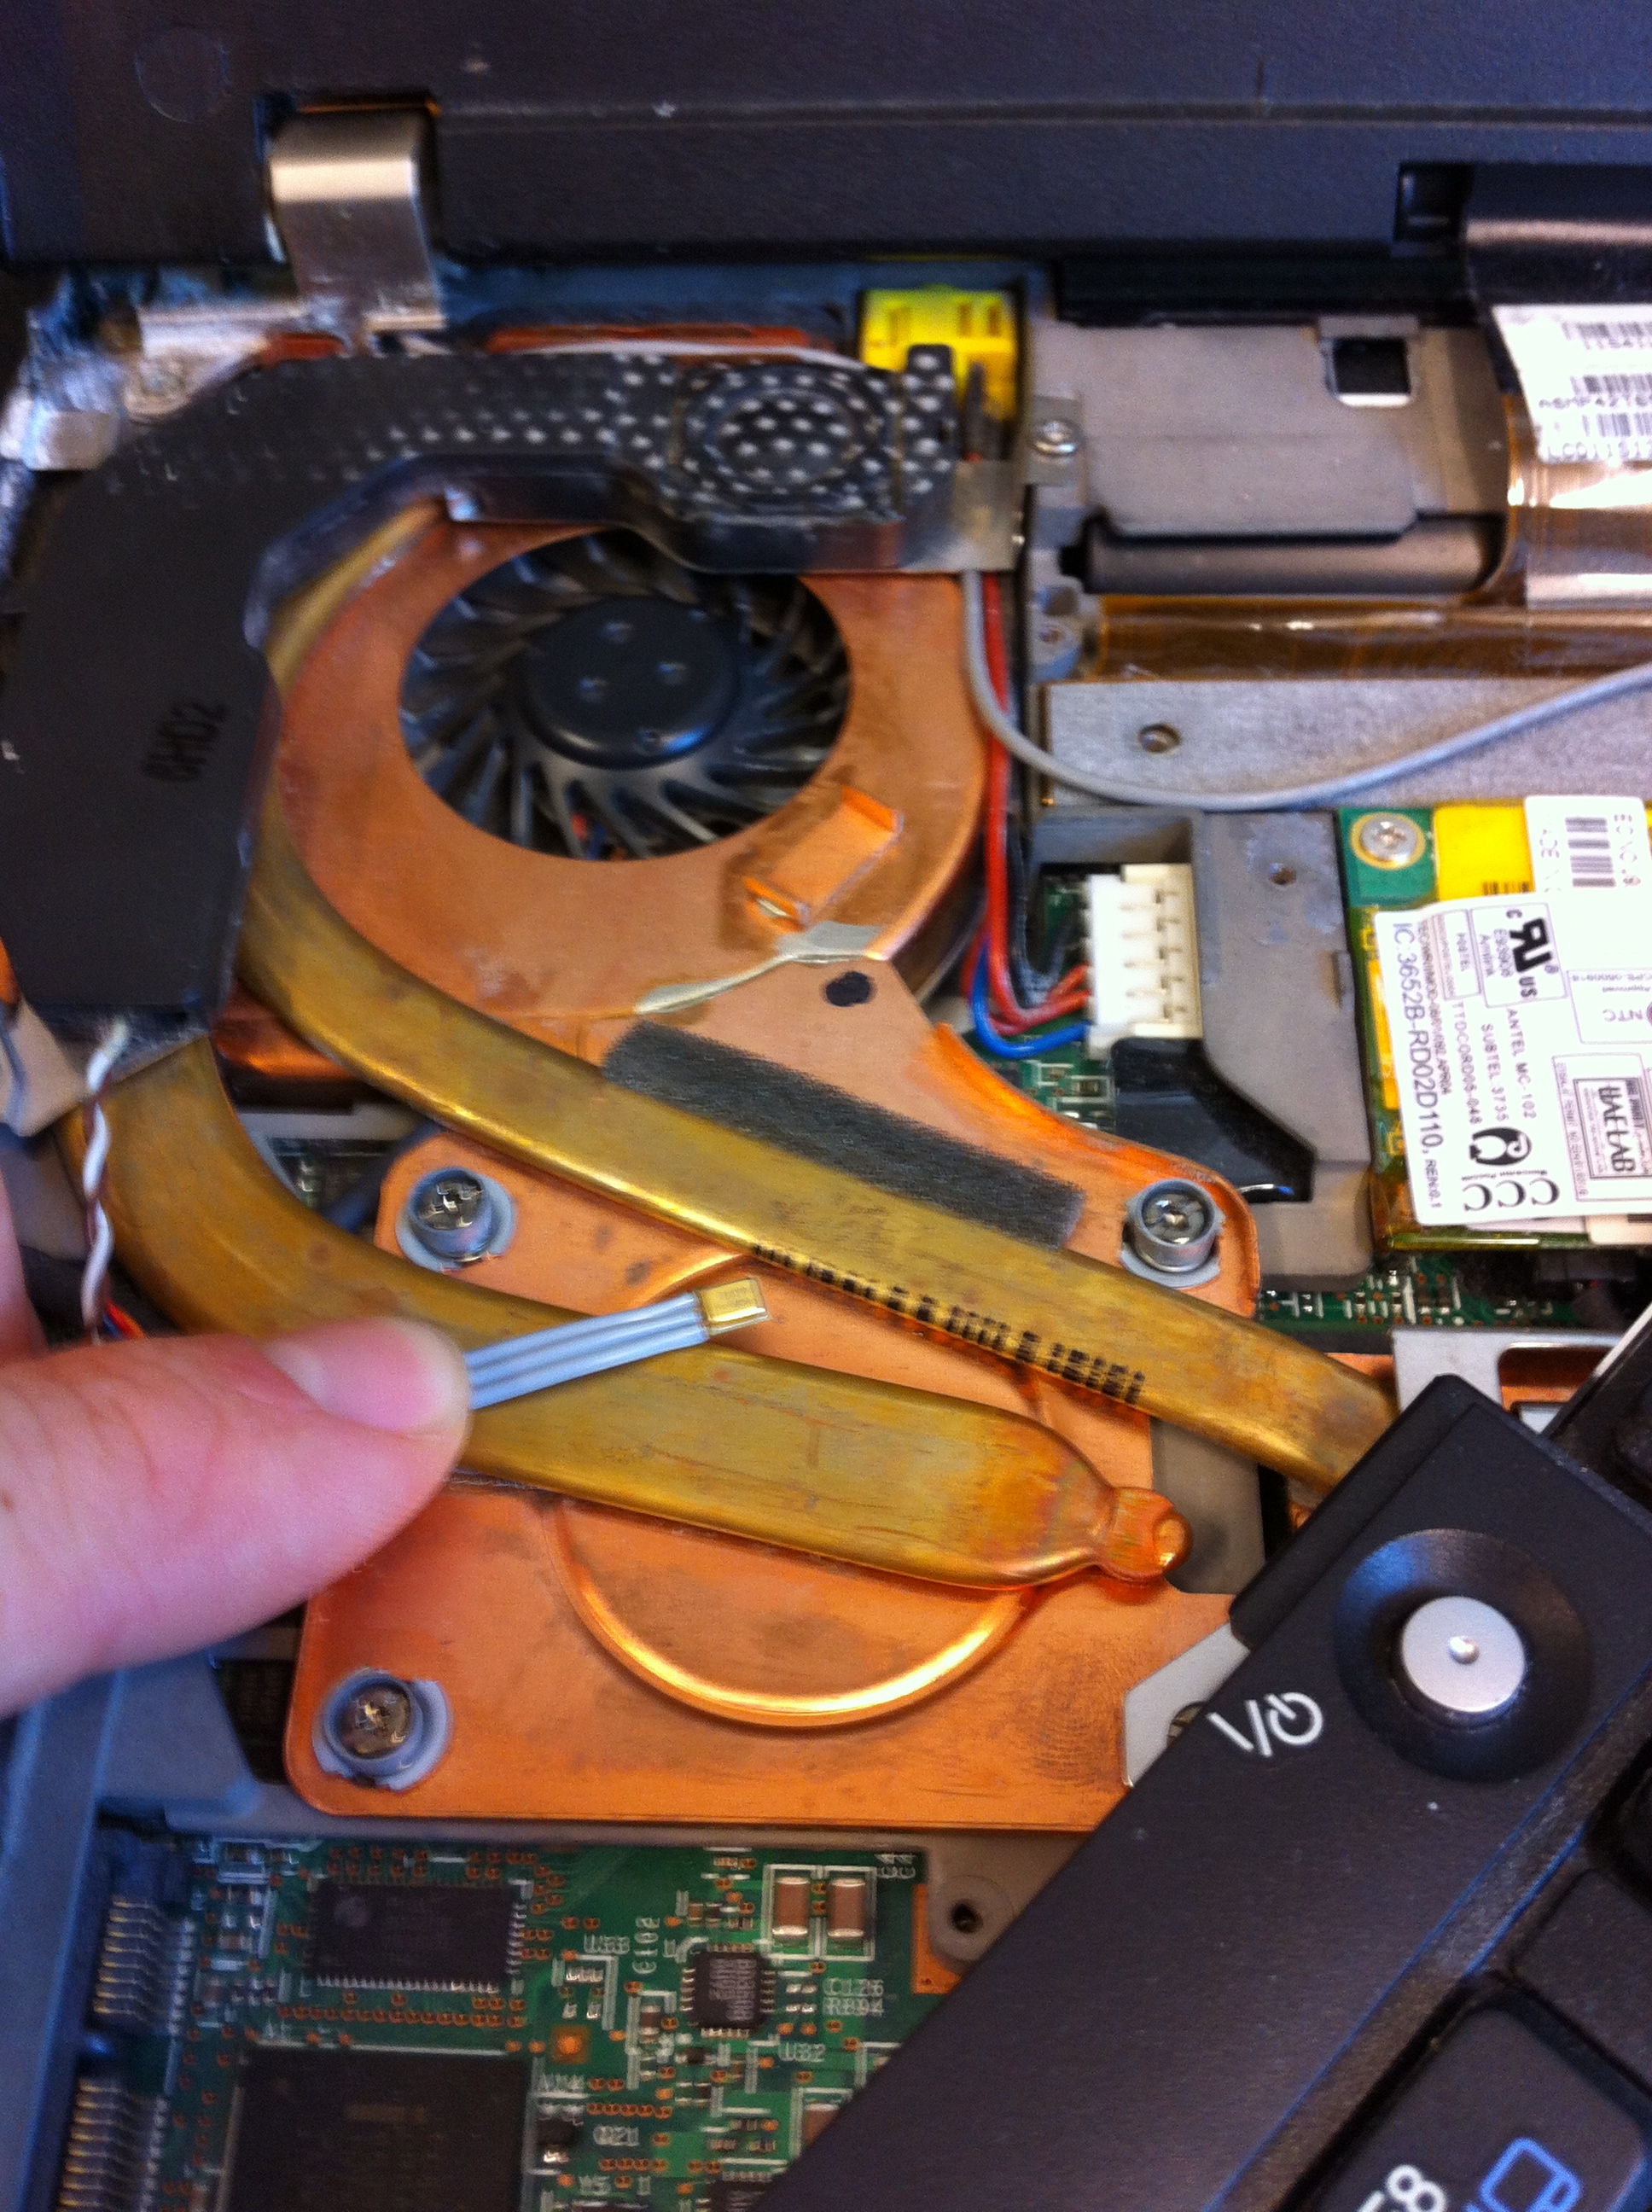
\includegraphics[width=0.5\textwidth]{T60p_knowles_position.JPG}
  \caption{A Knowles Ultrasonic SPU0410LR5H microphone positioned close to the CPU of a Lenovo T60p.}
  \label{fig:T60p_knowles_position}
\end{figure}

For the other target computers we use in the research, we strive to position the microphones as close to the CPU as possible, without breaking or dismantling the chassis.
A full list of all target computers and devices is given in \autoref{tbl:target_computers}.

\begin{table}[h]
  \begin{tabular}{lll}
  Computer                  & Operating System      & Processor                    \\ \hline
  Lenovo ThinkPad T60p      & 64-bit Linux Mint 17  & Intel Core 2 T7400 @ 2.16GHz \\ %\hline
  Dell Latitude D430        & 64-bit Linux Mint 17  & Intel Core 2 U7600 @ 1.20GHz \\ %\hline
  Raspberry Pi Model B      & Raspbian Wheezy       & ARM1176JZF-S @ 700MHz        \\ %\hline
  \end{tabular}
  \caption{Computers used during experiments.}
  \label{tbl:target_computers}
\end{table}

